\documentclass[12pt]{article}
\usepackage[T1]{fontenc}
\usepackage{float}
\usepackage{sbc-template}
\usepackage{graphicx,url}
\usepackage[brazil]{babel}   
\usepackage[utf8]{inputenc}  
\usepackage{indentfirst}
\usepackage{caption3}
\usepackage{color}
\usepackage{alltt}
\usepackage{url}
\usepackage{listings}

\lstset{ %
language=C,                % choose the language of the code
basicstyle=\footnotesize,       % the size of the fonts that are used for the code
numbers=left,                   % where to put the line-numbers
numberstyle=\footnotesize,      % the size of the fonts that are used for the line-numbers
stepnumber=1,                   % the step between two line-numbers. If it is 1 each line will be numbered
numbersep=7pt,                  % how far the line-numbers are from the code
backgroundcolor=\color{white},  % choose the background color. You must add \usepackage{color}
showspaces=false,               % show spaces adding particular underscores
showstringspaces=false,         % underline spaces within strings
showtabs=false,                 % show tabs within strings adding particular underscores
frame=single,           % adds a frame around the code
tabsize=2,          % sets default tabsize to 2 spaces
breaklines=true,        % sets automatic line breaking
breakatwhitespace=false,    % sets if automatic breaks should only happen at whitespace
escapeinside={\%*}{*)},          % if you want to add a comment within your code
extendedchars=true,
emph={%  
    set, pair, bool%
    },emphstyle={\bfseries},
morekeywords={set, pair}
literate={á}{{\'a}}1 {ã}{{\~a}}1 {é}{{\'e}}1
}
     
\sloppy

\title{siC: Uma linguagem baseada em C incluindo fila como tipo primitivo}

\author{Gabriella de Oliveira Esteves, 110118995}

\address{Departamento de Ciência da Computação - Universidade de Brasília}

\begin{document} 

\maketitle

%------------------------------------------------
\section{Objetivo}

Este trabalho visa projetar e construir uma nova linguagem chamada de siC - Structure in C, baseada na linguagem C. O siC acrescenta a estrutura de dados fila como tipo de dado primitivo e, para manipulá-la, adiciona certas operações próprias para tal.

%------------------------------------------------
\section{Introdução}

\indent Um compilador é um programa que recebe como entrada um código fonte e o traduz para um programa equilavente em outra linguagem \cite{book}. Ele pode ser dividido em sete fases, ilustrado na Figura \ref{fig:compilador}.

\begin{figure}[!ht]
  \centering
  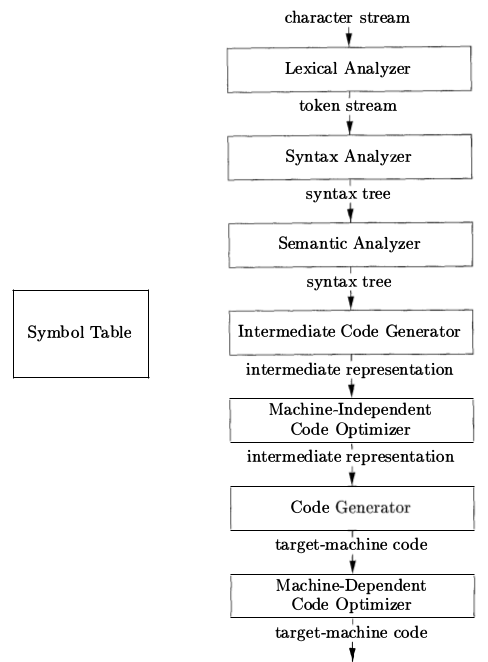
\includegraphics[width=0.5\textwidth]{compilador.png}
  \caption{Fases de um compilador} \label{fig:compilador}
\end{figure}

\begin{itemize}
	\item[1] \textbf{Analisador Léxico:} Lê o código fonte e atribui significado à cada sequência de caracteres, agora chamados lexemas. Cada lexema é mapeado para um token, que por sua vez é um par de nome (símbolo abstrato) e atributo (ponteiro para tabela de símbolos);
	\item[2] \textbf{Analisador Sintático:} Constrói uma representação gramatical dos tokens em forma de árvore;
	\item[3] \textbf{Analisador Semântico:} Utiliza a árvore sintática juntamente com a tabela de símbolos para verificar se a consistência semântica é mantida de acordo com a definição da linguagem.
	\item[4] \textbf{Gerador de Código Intermediário:} Converte árvore sintática anotada em código intermediário, com linguagem parecida com assembly e que possui apenas três operadores por linha de código. Nesse sentido, quebra-se estruturas complexas em estruturas mais simples, nesta fase.
	\item[5, 6] \textbf{Otimizador de Código Independente/Dependente de Máquina:} Procura aprimorar o código intermediário com o objetivo de melhorar o código-alvo de alguma forma: o deixando mais rápido, mais curto, consumindo menos energia, etc.
	\item[7] \textbf{Gerador de Código:} Converte o código intermediário no código-alvo, 	buscando atribuir os registradores às variáveis da maneira ótima.
\end{itemize}

\indent O foco do projeto será nas fase 1, 2, 3 e 4, porém a princípio serão apresentadas apenas a descrição da linguagem siC, uma breve descrição de sua semântica e o analisador léxico. Como a fila é uma das estruturas de dados mais básicas, é possível dizer que siC se destina a inúmeras áreas de Ciência da Computação, como, por exemplo, sistemas operacionais, onde ela é usada para organizar prioridades dos processos.

\indent Dois grandes motivos sustentam a escolha do tema deste projeto. Primeiro, uma vez que a fila faz parte dos tipos primitivos de uma linguagem, haverá menos manipulação de ponteiros na mesma, portanto erros envolvendo-os são menos prováveis de ocorrer. Segundo, a linguagem siC é mais alto-nível que C devido à abstração desta estrutura de dados básicas, e, de maneira geral, pode ser mais \textit{user-friendly}. Nesse sentido, o usuário (da linguagem) leigo deverá entender como a estrutura funciona, bem como suas vantagens/desvantagens e usabilidade; porém a implementação de cada uma estará a cargo da própria siC. 

\section{Gramática}

\indent A seguir será apresentada a gramática da linguagem siC, baseada em C \cite{yacc}. Alguns comentários são feitos ao longo da gramática para facilitar o entendimento das variáveis e nomenclatura utilizada. As palavras reservadas da linguagem são representadas aqui como \textit{tokens}. As variáveis e constantes são representadas como \textit{identifiers}, que por sua vez é uma expressão regular, e a única diferença entre este e \textit{identifier\_struct} é que o segundo tem acesso ao início da fila caso este seja o tipo do \textit{identifier}. 

\indent Antes de apresentá-la, segue abaixo algumas alterações e correções da versão passada deste arquivo:

\begin{itemize}
	\item[1] As variáveis \textit{argument}, \textit{compare\_expression} e \textit{type\_queue} foram removidas para aumentar a simplicidade da gramática, uma vez que elas possuiam apenas uma regra;
	\item[2] As variáveis \textit{arguments}, \textit{identifier\_struct\_expression}, \textit{statement} e \textit{statements} foram renomeadas para \textit{argList}, \textit{type\_struct\_expression}, \textit{stmt} e \textit{stmtList} respectivamente, para aumentar a legibilidade da gramática;
	\item[3] As variáveis \textit{identifiers}, \textit{identifier}, \textit{identifier\_struct}, \textit{caractere}, \textit{letra} e \textit{digito} foram removidas pois estes valores vêm direto do analisador léxico, atribuídos à nova variável chamada \textit{value};
	\item[4] Foi criada uma variável \textit{valueList} que permite, por exemplo, chamadas de função com mais de um parâmetro;
	\item[5] A variável \textit{statement} à direita das regras de IF, IF-ELSE e WHILE foram substituídas por \textit{block}. Um block representa apenas um \textit{statement} ou uma lista de \textit{statements} entre chaves;
	\item[6] As operações sobre dados do tipo fila foram substituídas de "+" para "SETLAST" e de "-" para "RMVFIRST" (Ver exemplo na Seção \ref{AnalSem});
	\item[7] Foram adiciondos os tokens EQ ("=="), NEQ ("!="), LEQ ("<="), GEQ (">="), LT ("<") e GT (">") para facilitar a passagem do lex para o bison.
\end{itemize}

Segue abaixo a gramática proposta cuja variável inicial é \textit{program}, com as alterações acima em vermelho e as características diferenciais da linguagem siC em negrito.


\begin{alltt}{\footnotesize
token: WHILE, IF, ELSE, RETURN, {\color{red}SETLAST}, {\color{red}RMVFIRST}
token: QUEUE, FIRST, VOID, FLOAT, INT, CHAR
token: {\color{red}EQ, NEQ, LEQ, GEQ, LT, GT}

{\color{red}program
   \(\to\) program function
   | function}

function
   \(\to\) {\color{red}type\_struct ID} ( argList ) \{ stmtList RETURN identifier ; \}
    
{\color{red}valueList
	\(\to\) valueList , value
	| value
	| \(\varepsilon\)}
	
}\end{alltt}
\indent Existe um novo tipo de dado, \textit{QUEUE}, que será composto por tipos simples de dados apenas (ou seja, não será possível criar uma variável do tipo fila em que seus elementos também são filas). Caso a variável seja do tipo fila, ela poderá obter o primeiro elemento através do comando "ID.FIRST".
\begin{alltt}{\footnotesize    	
	
{\color{red}value
	\(\to\) NUM\_INT
	| NUM\_FLOAT
	| CARACTERE
	| ID
	| ID . FIRST}
	
type\_struct
   \(\to\) type\_simple
    | \color{red}{QUEUE GT type\_simple LT}
    
type\_simple
   \(\to\) VOID | FLOAT | INT | CHAR  

argList
   \(\to\) argList , {\color{red}type\_struct ID}
   | {\color{red}type\_struct ID}
   | \(\varepsilon\)

   
}\end{alltt}
\indent A seguir serão descritas quatro estruturas básicas da linguagem siC: comando com repetição, condicional, expressões matemáticas e expressões com pilhas e filas. A última contempla as operações de adicionar elemento no topo da pilha ou no fim da fila, "SETLAST", e remover do topo ou do início da fila, "RMVFIRST", onde o valor do elemento retirado é armazenado no último operando da expressão.
\begin{alltt}{\footnotesize

stmtList
   \(\to\) stmtList stmt
   | \(\varepsilon\)

stmt
   \(\to\) {\color{red}type\_struct ID ;}
    | ID ( {\color{red}valueList} ) ;
    | ID = ID ( {\color{red}valueList} ) ;
    | IF ( {\color{red}value compare\_assignment value} ) {\color{red}block}
    | IF ( {\color{red}value compare\_assignment value} ) {\color{red}block} ELSE {\color{red}block}
    | WHILE ( {\color{red}value compare\_assignment value} ) {\color{red}block}
    | ID = assignment\_expression ;
    | \textbf{type_struct_expression}
    
{\color{red}block
	 \(\to\) stmt
    | \{ stmtList \} }
    
compare\_assignment
   \(\to\) {\color{red}EQ | NEQ | LEQ | GEQ | LT | GT}

assignment\_expression
   \(\to\) assignment\_expression + term
    | assignment\_expression - term
    | term
    
term
   \(\to\) term * factor
    | term / factor
    | factor
    
factor
   \(\to\) {\color{red}value}
    | ( assignment\_expression )
    
\textbf{
type\_struct_expression\
   \(\to\) ID = ID {\color{red}. SETLAST ARROW value} ;
    | ID = ID {\color{red}. RMVFIRST} ;
}		
}\end{alltt}

\section{Analisador Léxico}

\indent A principal tarefa do analisador léxico é examinar cada elemento do código fonte (variáveis, símbolos, números, etc), reconhecê-los com base em certos \textit{tokens} e classificá-los em grupos de lexemas. Além disso, ele pode realizar outras funções como eliminar espaços em brancos, tabulações, quebras de linhas e comentários; armazenar e acompanhar os números da linha e  coluna corrente no momento de sua execução; Informar mensagens de erro ou avisos de prevenção de erro diretamente ao usuário da linguagem \cite{book}.

\indent Existem três termos distintos bastante relacionados com analisador léxico. O primeiro, já citado anteriormente, é o \textit{token}, um par onde o primeiro elemento é o \textit{token name} (símbolo abstrato que representa um tipo de unidade léxica, como a palavra chave "while", por exemplo) e onde o segundo elemento é um atributo (informação adicional e opcional sobre o \textit{token}). O segundo termo é o \textit{pattern}, uma descrição, em forma de expressão regular, do um lexema de um token. No caso de um número inteiro, por exemplo, o \textit{pattern} seria uma sequência de um ou mais dígitos de 0 à 9. Por fim, o termo lexema significa uma sequência de caracteres no programa fonte que correspondem com o \textit{pattern} de um lexema específico, ou seja, cada lexema é uma instância de um token. No caso de existirem mais de uma correspondência, o lexema será a instância do \textit{token} cujo \textit{pattern} aparece primeiro no arquivo .lex.

\indent Esta seção apresenta o analisador léxico FLEX, utilizado neste trabalho, além de toda a descrição do arquivo .lex contruído a partir da gramática descrita no capítulo anterior.

\subsection{FLEX: The Fast Lexical Analyzer}

\indent Flex é uma ferramenta que gera um programa, chamado de \textit{scanner}, cuja função é identificar \textit{patterns} no código fonte. Ele recebe como entrada um arquivo de entrada especificados pelo usuário que serão reconhecidos a partir de expressões regulares mescladas com código em C (chamadas de descrição) no arquivo .lex \cite{flex}. Com o comando \textit{Flex nome\_do\_arquivo.lex}, um código fonte chamado \textit{lex.yy.c} é criado e nele existe uma função chamada \textit{yylex()}, a qual realiza de fato as operações do \textit{scanner}. Esse código, ao ser compilado corretamente com a flag \textit{-lfl} da biblioteca do flex, gera um arquivo objeto executável que recebe uma entrada qualquer e gera uma saída que depende do código em C que foi escrito no .lex (imprimir o lexema identificado, contabilizar o número de linhas, imprimir mensagem de erro léxico, etc).

\indent Neste projeto foram utilizadas duas variáveis globais muito úteis: \textit{yytext} e \textit{yyin}. A primeira contém o lexema que foi reconhecido como \textit{token}. Esta variável é modificada sempre que um novo lexema é identificado no código fonte. A segunda define como a entrada será lida, que pode ser tanto pela entrada padrão quanto por arquivo.



\begin{table}
 \centering
 \begin{tabular}{|c || c  l |} 
 \hline
   & \textit{Pattern} & Ação \\ [0.5ex] 
 \hline \hline
 1 & $\backslash$n	& Identifica uma quebra de linha e incrementa \\&& variável \textit{lines} para contagem de linhas \\ 
 \hline
 2 & [ $\backslash$t]+ 	& Identifica um ou mais espaço ou tabulação\\
 \hline
 3 & "//"[$\wedge\backslash$n]* & Ignora tudo a frente do comentário de \\&& uma linha "//" exceto quebra de linha \\
 \hline
 4 & \{digito\}+\{letra\}+\{digito\}* & {\color{red}Gera o erro identificado na linha \textit{lines}:} \\&& {\color{red}Sufixo inválido no número inteiro} \\
 \hline
 5 & {\footnotesize \{digito\}+"."\{digito\}*\{letra\}+\{digito\}*} & {\color{red}Gera o erro identificado na linha \textit{lines}:} \\&& {\color{red}Sufixo inválido no número float} \\
 \hline
 6 & \{digito\}+"."\{digito\}* & Identifica números float\\
 \hline
 7 & \{digito\}+ & Identifica números inteiros\\
 \hline
 8 & "'"(\{letra\}|\{digito\})"'" & Identifica valor para uma variável do \\&& tipo char, que pode ser uma letra ou dígito\\
 \hline
 9 & "''" & {\color{red}Gera o erro identificado na linha \textit{lines}:} \\&& {\color{red}Constante de caractere vazia} \\
 \hline 
 10 & "==", "!=", "<=", ">=", "<", ">" & Identifica símbolos de comparação \\&& entre dois elementos \\
 \hline
 11 & ".", ";", ",", "'", "\{", "\}", "(", ")" & Identifica pontuação e delimitadores de \\&& blocos e valores de char\\
 \hline
 12 & "+", "-", "*", "/" & Identifica operadores matemáticos \\
 \hline
 13 & (?i:"VOID")& Identifica palavra chave tipo void \\&& com as letras em caixa-alta ou caixa-alta. \\
 \hline
 14 & (?i:"FLOAT")& Identifica palavra chave tipo float \\&& com as letras em caixa-alta ou caixa-alta \\
 \hline
 15 & (?i:"INT")& Identifica palavra chave tipo inteiro \\&& com as letras em caixa-alta ou caixa-alta \\
 \hline
 16 & (?i:"CHAR") & Identifica palavra chave tipo char \\&& com as letras em caixa-alta ou caixa-alta \\
 \hline
 17 & (?i:"QUEUE")& Identifica palavra chave tipo fila \\&& com as letras em caixa-alta ou caixa-alta \\
 \hline
 18 & (?i:"FIRST")& Identifica palavra chave que representa \\&&  primeiro elemento da fila com as letras em \\&& caixa-alta ou caixa-alta  \\
 \hline
 19 & (?i:"IF")& Identifica palavra chave condicional if \\&& com as letras em caixa-alta ou caixa-alta \\
 \hline
 20 & (?i:"ELSE")& Identifica palavra chave condicional else \\&& com as letras em caixa-alta ou caixa-alta \\
 \hline
 21 & (?i:"WHILE")& Identifica palavra chave do laço while \\&& com as letras em caixa-alta ou caixa-alta \\
 \hline
 22 & (?i:"RETURN")& Identifica palavra chave return, de retorno de \\&& função, com as letras em caixa-alta ou caixa-alta \\
 \hline
 23 & \{id\} & Reconhece um identificador cuja regra é: não é \\&& permitido conter símbolos além de \$, letras e  dígitos \\&& e não é permitido começar a palara com dígito \\
 \hline
 24 & . & {\color{red}Gera o erro identificado na linha \textit{lines}:} \\&& {\color{red}\textit{Token} desconhecido} \\
 \hline
\end{tabular}
\caption{Tabela de regras}
\label{TabelaRegras}
\end{table}


\subsection{Arquivo lex}

\indent O código fonte de extensão .lex é composto por três partes: definições, regras e código em C do usuário. Na seção de definições é onde são declarados nomes para certas expressões regulares, para facilitar a escrita das regras na próxima seção. Neste projeto foram feitas seis definições, apresentadas na Tabela \ref{TabelaDef}. A primeira representa um dígito apenas, de 0 à 9. A segunda é uma letra maiúscula ou minúscula e o símbolo \$, que em C pode compor o nome de um identificador. A terceira representa os símbolos de comparação entre dois números elementos (que serão do tipo char, inteiro e float). A quarta representa delimitadores do código siC, para finalizar um comanto, definir um escopo, etc. A quinta definição apresenta as quatro operações matemáticas básicas. A sexta e última apresenta uma expressão regular que especifica o formato de um identificador: ele deve começar com uma letra ou \$ e pode terminar com letras, \$s ou dígitos.

\begin{table}
 \centering
 \begin{tabular}{| c || r  c |}
  \hline
   & Nome & Definição \\
  \hline  \hline
  1 & digito & [0-9] \\
  \hline
  2 & letra & [a-zA-Z\$] \\
  \hline
  6 & id & [a-zA-Z\$][a-zA-Z\$0-9]* \\
  \hline
\end{tabular}
\caption{Tabela de definições}
\label{TabelaDef}
\end{table}
 
\indent A segunda parte do código lex é composto pelas regras que são um par de \textit{pattern} e ação que devem estar na mesma linha. A Tabela \ref{TabelaRegras} apresenta cada regra utilizada no projeto. No código fonte, todos os elementos da entrada que são identificados são imprimidos, exceto quebra de linha, espaços, tabulações e comentários, que são ignorados. Existem três variáveis contadoras que são utilizadas nas ações: \textit{lines}, que começa com um e é incrementada sempre que uma quebra de linha é reconhecida, e \textit{errors}, que começa com zero e é incrementada sempre que um erro léxico é encontrado. Ao longo da execução são imprimidos as descrições dos erros léxicos na tela e, ao final, o número total de erros.

\indent A ordem em que as regras estão é importante para o funcionamento correto do programa, pois se existir mais de uma correspondência de \textit{pattern} para um elemento, ele será identificado pela regra que aparecer primeiro. Neste projeto, as regras das keywords deve vir antes das regras dos identificadores, pois assim, se a seguinte entrada \textit{int x = 2;} for lida, por exemplo, o elemento \textit{int} será reconhecido como identificador e também tipo inteiro, porém a regra de keyword deverá identificá-lo.

\indent Os \textit{patterns} contidos entre chaves foram definidos na seção de descrição. Em relação aos demais, segue abaixo a descrição de algumas expressões regulares. 

\begin{itemize}
  \item[ [$\wedge\backslash$n] ] : Reconhece tudo exceto espaço e quebra de linha (Exemplo: regra 3);
  \item[\{digito\}] : Reconhece apenas um dígito (Exemplo: regra 8);
  \item[\{digito\}*] : Reconhece zero ou mais dígitos (Exemplo: regra 6);
  \item[\{digito\}+] : Reconhece um ou mais dígitos (Exemplo: regra 5);
  \item[``abc''] : Reconhece a sequência de caracteres "abc" (Exemplo: regra 9);
  \item[``a'' $\vert$ ``b''] : Reconhece o caractere "a" ou o "b" (Exemplo: regra 8);
  \item[(?i:"AB")] : Reconhece as sequências "AB", "Ab", "aB", "ab" (Exemplo: regra 13);
  \item[.] : Reconhece qualquer elemento (Exemplo: regra 24).
\end{itemize}

\indent A terceira parte do código lex é composta por código em C, que define como será lida a entrada (por arquivo ou pela entrada padrão) e define também as ações tomadas por cada \textit{pattern}.

\subsection{Erros Léxicos}

\indent Foram reconhecidos quatro erros léxicos em siC. Caso exista um elemento que comece com dígitos e termine com letras, o usuário será informado de que o sufixo de letras é inválido para um tipo inteiro (regra 4). Caso exista um elemento que comece com dígitos, tenha depois um ponto, e termine com letras, o usuário será informado de que o sufixo de letras é inválido para um tipo float (regra 5). Caso exista na entrada duas aspas simples, uma seguida da outra, o programa entende que entre eles deveria existir algum caractere que seria o valor que algum char, portanto o usuário será informado de que a constante de caractere está vazia (regra 9). Por fim, caso exista algum elemento não identificado na entrada, o usuário será informado (regra 24).

\indent Para testar o código foram criados dois arquivos de extensão .sic, um de acordo com as normas especificadas neste projeto (teste\_correto.sic), outro com todos os quatro tipos de erros léxicos (teste\_errado.sic). Cinco erros léxicos são reportados neste último arquivo:

\begin{itemize}
  \item[1] \textbf{ERROR on line 4 : Invalid suffix on integer ``0i0''} \\ Erro de variável começando começando com dígito, ou número inteiro contendo algum caractere;
  \item[2] \textbf{ERROR on line 9 : Invalid suffix on floating ``0.0a0''} \\ Erro de número float contendo algum caractere;
  \item[3] \textbf{ERROR on line 16 : Unknown token '!'} \\  Erro de caractere desconhecido;
  \item[4] \textbf{ERROR on line 17 : Empty character constant `` `' ''} \\ Nesta linha ocorreu a inserção de um caractere vazio na pilha q;
  \item[5] \textbf{ERROR on line 21 : Unknown token '@'} \\ Outro erro de caractere desconhecido.
\end{itemize}

\subsection{Dificuldades enfrentadas}

\indent Nesta fase do projeto, as principais dificuldades foram construir as expressões regulares que formam os \textit{patterns}, bem como ordená-las de forma que o analisador respeite as regras de precedência de reconhecimento dos padrões. Além disso, foi um desafio procurar por erros léxicos, uma vez que os principais e mais conhecidos são sintáticos.






\section{Analisador Sintático}

\indent O analisador sintático recebe como entrada o retorno de cada elemento aprensentado na tabela \ref{TabelaRegras} do analisador léxico e constrói duas estrutura de dados: a árvore sintática, que representa a hierarquia do código e a tabela de símbolos, que apresenta os identificadores do programa. O parser escolhido para realizar o projeto foi gerado pelo Bison.

\subsection{GNU Bison: Parser Generator}

\indent O Bison é um gerador de Parser do tipo \textit{top-down} LALR(1) (\textit{Left-to-Right scanning, Rightmost derivation with Looahead}), escrito por Robert Corbett e Richard Stallman. A versão utilizada foi a 3.0.4. O Bison é uma implementação do YACC ("\textit{Yet another compiler-compiler}"), gerador de parser LALR com \textit{lookahead} também.

\subsection{Arquivo y e structs}

\indent A partir do projeto do analisador sintático foi necessário criar um \textit{Makefile} para ligar a biblioteca \textit{structs.h} e conectar os analisadores léxicos e sintáticos, portanto basta dar o comando \textit{make} para criar o executável e \textit{make clean} para limpar a pasta. \\

\indent Para representar cada variável da gramática, fez-se uma \textit{struct} chamada \textit{Variable} apresentada abaixo, onde o atributo \textit{variable\_name} é o nome da variável, \textit{variable\_tag} é seu identificador, \textit{variable\_num\_nexts} é a quantidade de filhos cuja regra selecionada da variável possui, \textit{token} é o próprio token passado do léxico para o sintático, \textit{rule\_num} é o identificador desta regra selecionada e \textit{variable\_list} é um ponteiro para uma lista de variáveis filhas da regra selecionada. \textit{MAX\_WORD} define um tamanho máximo para o nome de uma variável e o token (elementos não dependentes do usuário da linguagem siC) e \textit{MAX\_CHILD\_RULES} define o número máximo de filhos que uma regra pode possuir. \\
\begin{lstlisting}[language=C]
#define MAX_WORD 64
#define MAX_CHILD_RULES 5
typedef struct Variable {
    char variable_name[MAX_WORD];
    int variable_tag;
    int variable_num_nexts;
    char token[MAX_WORD];
    int rule_num;
    struct Variable *variable_list[MAX_CHILD_RULES];
} Variable;
}
\end{lstlisting}
\indent A gramática está localizada no arquivo 110118995.y, agora com ações semânticas sempre ao final de cada regra. As variável foram definidas como sendo do tipo \textit{Variable} e os demais \textit{tokens}, do tipo \textit{string}. Todas as ações semânticas fazer o mesmo: um vetor de x \textit{structs} \textit{varList} é alocado na memória, onde x é o número de filhos que aquela regra possui. O ponteiro para cada filho (representados por \$x). é atribuído para \textit{varList[i] }e, por fim, a função para criar uma nova variável é chamada e seu retorno é atribuído à variável cuja regra está sendo executada (representada por \$\$). Os parâmetros desta função, \textit{new\_variable}, são (1) a tag da variável, (2) número de filhos que a regra possui, (3) a lista de variáveis para as quais ela aponta, (4) um terminal da regra, (5) o identificador da regra para aquela variável. Quando a regra possui algum token, ele é adicionado à tabela de símbolos na ação semântica também (função \textit{add\_symbol\_on\_table} é chamada). A função de criar nova variável está localizada no arquivo structs.h, assim como a \textit{struct Variable} e as funções de mostrar a árvore sintática, adicionar um elemento na tabela de símbolos e mostrar a tabela de símbolos.  \\

\indent A função \textit{new\_variable} apenas alloca espaço para uma \textit{struct Variable} e passa os elementos do parâmetro para os atributos da \textit{struct}. Para cada variável, é atribuído dentro de um \textit{switch-case} seu nome, tag e, quando necessário, o \textit{token}. A função \textit{add\_symbol\_on\_table} adiciona um terminal passado por parâmetro à um vetor de strings global, se este terminal ainda não está presente no vetor. A função \textit{show\_symbol\_table} percorre este vetor ao final do programa, imprimindo na tela todos os terminais.

\subsection{Árvore sintática}
\indent A árvore sintática foi construída ao longo da leitura da entrada, pois cada ação semântica cria novos nós de baixo para cima. Nesse sentido, a impressão da árvore poderia ser feita inversamente nas ações semânticas, porém, por questões de estética, foi feito uma função \textit{show\_tree} para tal. Ela é chamada pela primeira regra da variável inicial da gramática (topo da árvore) e recebe como parâmetro um nó de \textit{Variable}, o número de \textit{tabs} necessárias para a impressão de uma árvore legível e o índice do primeiro filho daquela regra (para facilitar a impressão na função recursiva). A função verifica se o \textit{token} daquele nó é vazio (identificado pela string "END"), ou algum operador matemático, significando que aquele nó é uma \textit{Variable} com filhos. Se ele é, então seu nome é impresso e em seguida os elementos que compõem aquela regra. Se ele possui filhos, a função \textit{show\_tree} é chamada recursivamente. Se ele não é, ou seja, se o nó é uma folha,  seu terminal é impresso.

\subsection{Erros Léxicos}

\subsection{Dificuldades enfrentadas}

\indent A principal dificuldade foi a criação da estrutura da árvore sintática. A princípio tentei construir uma \textit{struct} para cada variável, o que funcionou até o momento em que  foi necessário imprimir a árvore. Como não consegui percorrer uma árvore de várias structs diferentes, criei uma \textit{union} cujos atributos eram todas estas \textit{structs}, porém me deparei com um código gigante com vários pequenos erros e então resolvi começar tudo de novo com apenas uma string chamada \textit{Variable} que possui certos atributos desnecessários para algumas regras, porém aumenta a legibilidade do programa. \\

\indent Além disso, acredito que a impressão da árvore não estega correta da forma que está, pois a ordem com que os identificadores aparecem não está óbvia na função \textit{show\_tree}. As regras de escopo na tabela de símbolos não foram implementadas.

%\subsection{Árvore sintática}

%\subsection{Tabela de símbolos}

\section{Analisador Semântico} \label{AnalSem}

\indent A análise semântica utiliza da árvore sintática para checar a consistência da linguagem. Uma de suas obrigações mais importantes é a checagem de tipo. No caso do siC, existem várias restrições a serem consideradas:
\begin{itemize}
    \item Para adicionar um elemento A de tipo simples (char, int ou float) no fim da fila de um elemento struct B, a atribuição deve ser do tipo B = B + A, onde A deverá ter tipo compatível com o de B, ou seja, se B for fila de inteiros, A deve ser um inteiro;
    \item Para remover um elemento A de tipo simples (char, int ou float) do início da fila de um elemento struct B, a atribuição deve ser do tipo B = B - A, onde A deverá ter tipo compatível com o de B, ou seja, se B for fila de inteiros, A deve ser um inteiro;
    \item Nenhuma operação matemática (\textit{assignment\_expression}) pode conter um identificador B do tipo fila, apenas seu início, ou seja, B.FIRST.
\end{itemize}

\indent Um exemplo de código em siC é aprensentado a seguir. O programa adiciona três elementos numa fila de inteiros e depois eles são somados um a um e armazenados na variável \textit{sum}. Ao final, a variável \textit{lixo}, recém retirada da fila, é adicionada à \textit{sum}. Nesse sentido, o resultado final de sum deve ser 7. \\

\begin{lstlisting}[language=C]
VOID main () {
    QUEUE<INT> q;
    INT sum, INT lixo;

    q = q + 0;
    q = q + 1;
    q = q + 2;
    q = q + 3;    
    sum = 0;
    
    WHILE (q.FIRST != 0) {    
        sum = (sum + q.FIRST);
        q = q - lixo;
    }
    sum = sum + lixo;

    RETURN 0;
}

\end{lstlisting}

%\section{Geração de código intermediário}

% \section{Considerações finais}

\begin{thebibliography}{1}
\bibitem{book}
A.~V.~Abo, M.~S.~Lam, R.~Sethi, J.~D.~Ullman, \emph{Compilers - Principles, Techniques and Tools}
\hskip 1em plus
	0.5em minus 0.4em\relax 2nd ed. 1986
	
\bibitem{yacc}
ANSI C Yacc grammar, \url{http://www.quut.com/c/ANSI-C-grammar-y.html}, 18 12 2012.

\bibitem{flex}
Flex: The Fast Lexical Analyser, \url{http://flex.sourceforge.net/}, The Flex Project, 2008
\end{thebibliography}
%------------------------------------------------
\end{document}